\chapter{Risk Propagation}\label{ch:risk-propagation}

Risk propagation is a message-passing algorithm that estimates an individual's infection risk by considering their demographics, symptoms, diagnosis, and contact with others. Formally, a \define{risk score} $\vScore_t$ is a timestamped infection probability where $\vScore \in [0, 1]$ and $t \in \naturals$ is the time of its computation. Thus, an individual with a high risk score is likely to test positive for the infection and poses a significant health risk to others. There are two types of risk scores: \define{symptom scores}, or prior infection probabilities, which account for an individual's demographics, symptoms, and diagnosis \citep{Menni2020}; and \define{exposure scores}, or posterior infection probabilities, which incorporate the risk of direct and indirect contact with others.

Given their recent risk scores and contacts, an individual's exposure score is derived by marginalizing over the joint infection probability distribution. Naively computing this marginalization scales exponentially with the number of variables (i.e., individuals). To circumvent this intractability, the joint distribution is modeled as a factor graph, and an efficient message-passing procedure is employed to compute the marginal probabilities with a time complexity that scales linearly in the number of factor nodes (i.e., contacts).

Let $\vGraph = (\vVariables, \vFactors, \vEdges)$ be a \define{factor graph} where $\vVariables$ is the set of variable nodes, $\vFactors$ is the set of factor nodes, and $\vEdges$ is the set of edges incident between them \citep{Kschischang2001}. 

A \define{variable node} $\vVariable: \eventSpace \rightarrow \{0, 1\} $ is a random variable that represents the infection status of an individual, where the sample space is $\eventSpace = \{\var{healthy}, \var{infected}\}$ and
\begin{equation*}
  \vVariable(\event) =
    \begin{cases}
      0 & \text{if } \event = \var{healthy} \\
      1 & \text{if } \event = \var{infected}.
    \end{cases}
\end{equation*}
Thus, $\pr{\vVariable[i]}[t] = \vScore_t$ is a risk score of \indexed{i}{individual}.

A \define{factor node} $\vFactor: \vVariables \times \vVariables \rightarrow [0, 1]$ defines the transmission of infection risk between two contacts. Specifically, contact between \twoindexed{i}{j}{individual} is represented by the factor node $\vFactor(\vVariable[i], \vVariable[j])$ = $\vFactor[ij]$, which is adjacent to the variable nodes $\vVariable[i], \vVariable[j]$. This work and \citet{Ayday2021} assume risk transmission is a symmetric function, $\vFactor[ij] = \vFactor[ji]$. However, it may be extended to account for an individual's susceptibility and transmissibility such that $\vFactor[ij] \neq \vFactor[ji]$. \Cref{fig:factor-graph} depicts a factor graph that reflects the domain constraints.

\begin{figure}[htb]
\centering
\begin{tikzpicture}[ampersand replacement=\&]
  \matrix[row sep=1.5em, column sep=0.75em] {
    \& \factor[minimum size=1em] {f12} {above:$\vFactor[12]$} {} {}; \&\&
    \factor[minimum size=1em] {f23} {above:$\vFactor[23]$} {} {}; \& \\
    \node[latent, minimum size=2em] (v1) {$\vVariable[1]$}; \&\&
    \node[latent, minimum size=2em] (v2) {$\vVariable[2]$}; \&\&
    \node[latent, minimum size=2em] (v3) {$\vVariable[3]$}; \\
  };
  \edge[-] {v1} {f12};
  \edge[-] {v2} {f12};
  \edge[-] {v2} {f23};
  \edge[-] {v3} {f23};
\end{tikzpicture}
\caption[Factor graph]{A factor graph of 3 variable nodes and 2 factor nodes.}
\label{fig:factor-graph}
\end{figure}

\section{Synchronous Risk Propagation}\label{sec:synchronous}

\newcommand{\pDiff}{\epsilon}
\newcommand{\topK}[1]{\text{top } K \text{ of } #1}
\newcommand{\vRiskScores}[2]{\vSet{R}_{#1}^{(#2)}}
\newcommand{\vExposureScore}[2]{r_{#1}^{(#2)}}
\newcommand{\vExposureScores}[1]{\mathbf{r}^{(#1)}}
\newcommand{\dist}{d}

\citet{Ayday2021} first proposed risk propagation as a synchronous, iterative message-passing algorithm that uses the factor graph to compute exposure scores. The first input to \cRiskPropagation{} is the set family $\vScores$, where
\begin{equation} \label{eq:score-set}
  \vScores_i =\setBuilder{\vScore_t}{\vRefTime - t < \pScoreExpiry} \in \vScores
\end{equation}
is the set of recent risk scores of \indexed{i}{individual}. The second input to \cRiskPropagation{} is the contact set
\begin{equation} \label{eq:contact-set}
  \vContacts = \setBuilder{(i, j, t)}{i \neq j, \vRefTime - t < \pContactExpiry}
\end{equation}
such that $(i, j, t)$ is the \emph{most recent} contact between \twoindexed{i}{j}{individual} that occurred from time $t$ until at least time $t + \pMinContactDuration$, where $\pMinContactDuration \in \naturals$ is the \define{minimum contact duration}\footnote{While \citet{Ayday2021} require contact over a $\pMinContactDuration$-contiguous period of time, the Centers for Disease Control and Prevention \citeyearpar{CDC2021} account for contact over a 24-hour period.}. Naturally, risk scores and contacts have finite relevance, so \eqref{eq:score-set} and \eqref{eq:contact-set} are constrained by the \define{risk score expiry} $\pScoreExpiry \in \naturals$ and the \define{contact expiry} $\pContactExpiry \in \naturals$, respectively. The \define{reference time} $\vRefTime \in \naturals$ defines the relevance of the inputs and is assumed to be the time at which \cRiskPropagation{} is invoked. For notational simplicity in \cRiskPropagation{}, let $\vSomeSet$ be a set. Then $\max \vSomeSet = 0$ if $\vSomeSet = \emptyset$.

\subsection{Variable Messages}

The current exposure score of \indexed{i}{individual} is defined as $\max \vScores_i$. Hence, a \define{variable message} $\vVariableMessage{i}{j}{n}$ from the variable node $\vVariable[i]$ to the factor node $\vFactor[ij]$ during \indexed{n}{iteration} is the set of maximal risk scores $\vRiskScores{i}{n - 1}$ from the previous $n - 1$ iterations that were not derived by $\vFactor[ij]$. In this way, risk propagation is reminiscent of the max-sum algorithm; however, risk propagation aims to maximize \emph{individual} marginal probabilities rather than the joint distribution \cite[pp. 411--415]{Bishop2006}.

\subsection{Factor Messages}

A \define{factor message} $\vFactorMessage{i}{j}{n}$ from the factor node $\vFactor[ij]$ to the variable node $\vVariable[j]$ during \indexed{n}{iteration} is an exposure score of \indexed{j}{individual} that is based on interacting with those at most $n - 1$ degrees separated from \indexed{i}{individual}. This population is defined by the subgraph induced in $\vGraph$ by
\begin{equation*}
  \setBuilder{v \in \vVariables \cap \vFactors \setminus \{\vVariable[j], \vFactor[ij]\}}{\dist(\vVariable[i], v) \leq 2(n - 1)},
\end{equation*}
where $\dist(u, v)$ is the distance between the nodes $u, v$. The computation of a factor message assumes the following.
\begin{enumerate}
  \item Contacts have a nondecreasing effect on an individual's exposure score.
  \item A risk score $\vScore_t$ is \define{relevant} to the contact $(i, j, t_{ij})$ if $t < t_{ij} +\pTimeBuffer$, where $\pTimeBuffer \in \naturals$ is a \define{time buffer} that accounts for the incubation period, along with the delayed reporting of symptom scores and contacts. The expression $t_{ij} +\pTimeBuffer$ is called the \define{buffered contact time}.
  \item Risk transmission between contacts is incomplete. Thus, a risk score decays exponentially along its transmission path in $\vGraph$ at a rate of $\log \pTransmissionRate$, where $\pTransmissionRate \in (0, 1)$ is the \define{transmission rate}.
\end{enumerate}
To summarize, a factor message $\vFactorMessage{i}{j}{n}$ is the maximum relevant risk score in the variable message $\vVariableMessage{i}{j}{n}$ (or 0) that is scaled by the transmission rate $\pTransmissionRate$.

\citet{Ayday2021} assume that the contact set $\vContacts$ may contain (1) multiple contacts between the same two individuals and (2) \define{invalid} contacts, or those lasting less than $\pMinContactDuration$ time. However, these assumptions introduce unnecessary complexity. Regarding assumption 1, suppose \twoindexed{i}{j}{individual} come into contact $m$ times such that $t_k < t_\ell$ for $1 \leq k < \ell \leq m$. Let $\vFactorMessages_k$ be the set of relevant risk scores, according to the contact time $t_k$, where
\begin{equation*}
  \vFactorMessages_k = \setBuilder{\pTransmissionRate \vScore_t}{\vScore_t \in \vVariableMessage{i}{j}{n}, t < t_k + \pTimeBuffer}.
\end{equation*}
Then $\vFactorMessages_k \subseteq \vFactorMessages_\ell$ if and only if $\max \vFactorMessages_k \leq \max \vFactorMessages_\ell$. Therefore, only the most recent contact time $t_m$ is required to compute the factor message $\vFactorMessage{i}{j}{n}$. With respect to assumption 2, there are two possibilities.
\begin{enumerate}
  \item If an individual has at least one valid contact, then their exposure score is computed over the subgraph induced in $\vGraph$ by their contacts that define the neighborhood $\vNeighbors_i$ of the variable node $\vVariable_i$.
  \item If an individual has no valid contacts, then their exposure score is $\max \vScores_i$ or $0$, if all of their previously computed risk scores have expired.
\end{enumerate}
In either case, a set $\vContacts$ containing only valid contacts implies fewer factor nodes and edges in the factor graph $\vGraph$. Consequently, the complexity of \cRiskPropagation{} is reduced by a constant factor since fewer messages must be computed.

\subsection{Termination}

To detect convergence, the normed difference between the current and previous exposure scores is compared to the threshold $\pDiff \in \reals$. Note that $\vExposureScores{n}$ is the vector of exposure scores in the \indexed{n}{iteration} such that $\vExposureScore{i}{n}$ is \indexed{i}{component} of $\vExposureScores{n}$. The $\ell^1$ and $\ell^\infty$ norms are sensible choices for detecting convergence. \citet{Ayday2021} use the $\ell^1$ norm, which ensures that an individual's exposure score changed by at most $\pDiff$ after the penultimate iteration.

\begin{function}[H]{\nRiskPropagation}[\vScores, \vContacts]
  \State $(\vVariables, \vFactors, \vEdges) \assign \cCreateFactorGraph[\vContacts]$
  \State $n \assign 1$
  \ForEach{$\vVariable[i] \in \vVariables$}
    \State $\vRiskScores{i}{n - 1} \assign \topK{\vScores_i}$
    \State $\vExposureScore{i}{n - 1} \assign \max \vRiskScores{i}{n - 1}$
    \State $\vExposureScore{i}{n} \assign \infty$
  \EndFor
  \While{$\| \vExposureScores{n} - \vExposureScores{n - 1} \| > \pDiff$}
    \ForEach{$\{\vVariable[i], \vFactor[ij]\} \in \vEdges$}
      \State $\vVariableMessage{i}{j}{n} \assign \vRiskScores{i}{n - 1} \setminus \setBuilder{\vFactorMessage{j}{i}{k}}{k \in [1 \twodots n - 1]}$
    \EndFor
    \ForEach{$\{\vVariable[i], \vFactor[ij]\} \in \vEdges$}
      \State $\vFactorMessage{i}{j}{n} \assign \max \setBuilder{\pTransmissionRate \vScore_t}{\vScore_t \in \vVariableMessage{i}{j}{n}, t < t_{ij} + \pTimeBuffer}$
    \EndFor
    \ForEach{$\vVariable[i] \in \vVariables$}
      \State $\vRiskScores{i}{n} \assign \topK{\setBuilder{\vFactorMessage{j}{i}{n}}{\vFactor[ij] \in \vNeighbors_i}}$
    \EndFor
    \ForEach{$\vVariable[i] \in \vVariables$}
      \State $\vExposureScore{i}{n - 1} \assign \vExposureScore{i}{n}$
      \State $\vExposureScore{i}{n} \assign \max \vRiskScores{i}{n}$
    \EndFor
    \State $n \assign n + 1$
  \EndWhile
  \State \Return $\vExposureScores{n}$
\end{function}

\section{Asynchronous Risk Propagation}\label{sec:asynchronous}

While straightforward to specify, \cRiskPropagation{}, is not a viable implementation for real-world application, because it is an \define{offline algorithm} that requires all individuals' recent contacts and risk scores to run. As \citet{Ayday2021} note, the centralization of health and contact data is not privacy preserving. An offline design is also computational inefficient and risks human safety. Specifically, most exposure scores may not change across invocations of \cRiskPropagation{}, which implies communication overhead and computational redundancy. As a mitigation, \citet{Ayday2020} suggest running \cRiskPropagation{} only once or twice daily. However, this causes substantial delay in reporting to individuals their exposure scores; and in the face of a pandemic, timely information is essential for individual and collective health.

To address the privacy limitations of \cRiskPropagation{}, \citet{Ayday2021} propose decentralizing the factor graph such that the processing entity (e.g., mobile device or ``personal cloud'') associated with \indexed{i}{individual} maintains the state of \indexed{i}{variable node} and its neighboring factor nodes. But for real-world application, the proposal leaves key questions unanswered:
\begin{enumerate}
  \item Is message passing synchronous or asynchronous?
  \item How does message passing terminate?
  \item Are any optimizations utilized to reduce communication cost?
  \item How do processing entities exchange messages over the network?
  \item How private is decentralized risk propagation?
\end{enumerate}

%Key observations:
%
%- Asynchronous message passing amongst stateful entities is the essence of the actor model, so we can use it to describe risk propagation as an online algorithm
%- By applying one-mode projection, the factor graph is equivalent to a contact network. Thus, we can extend the concepts of reachability in temporal network to account for message-passing semantics and measure the communication complexity of risk propagation.

The only purpose of a factor node is to compute and relay messages between variable vertices. Thus, one-mode projection onto the variable vertices can be applied such that variable vertices $\vVariable[i],\vVariable[j] \in \vVariables$ are adjacent if the factor node $\vFactor[ij] \in \vFactors$ exists \citep{Zhou2007}. \Cref{fig:projected} shows the modified topology.

\begin{figure}[htb]
\centering
\begin{tikzpicture}[ampersand replacement=\&]
  \matrix[row sep=7em, column sep=2em] {
    \node[latent, minimum size=2em] (v1) {$\vVariable[1]$}; \&\&\&
    \node[latent, minimum size=2em] (v2) {$\vVariable[2]$}; \&\&\&
    \node[latent, minimum size=2em] (v3) {$\vVariable[3]$}; \\
  };
  \factor[minimum size=1em, above= of v1] {f12_1} {above:$\vFactor[12]$} {} {};
  \factor[minimum size=1em, above= of v2, xshift=-3em] {f12_2} {above:$\vFactor[12]$} {} {};
  \factor[minimum size=1em, above= of v2, xshift=3em] {f23_2} {above:$\vFactor[23]$} {} {};
  \factor[minimum size=1em, above= of v3] {f23_3} {above:$\vFactor[23]$} {} {};
  
  \plate{p1} {(v1)(f12_1)(f12_1-caption)} {};
  \plate{p2} {(v2)(f12_2)(f23_2)(f12_2-caption)(f23_2-caption)} {};
  \plate{p3} {(v3)(f23_3)(f23_3-caption)} {};
  
  \edge[-] {v1} {f12_1};
  \edge[-] {v2} {f12_2};
  \edge[-] {v2} {f23_2};
  \edge[-] {v3} {f23_3};
  \edge[-] {p1} {p2};
  \edge[-] {p2} {p3};
\end{tikzpicture}
\caption[One-mode projection of a factor graph]{One-mode projection onto the variable nodes in \Cref{fig:factor-graph}.}
\label{fig:projected}
\end{figure}

To send a message to variable node $\vVariable[i]$, variable node $\vVariable[j]$ applies the computation associated with the factor node $\vFactor[ij]$. This modification differs from the distributed extension of risk propagation \citep{Ayday2021} in that we do not create duplicate factor vertices and messages in each user's PDS. By storing the contact time between users on the edge incident to their variable vertices, this modified topology is identical to the \define{contact-sequence} representation of a \define{contact network}, a kind of \define{temporal network} in which a node represents a person and an edge indicates that two persons came in contact:
\begin{equation}
  \setBuilder{(u, v, t)}{u, v \in \vVertices; u \neq v; t \in \naturals}, \label{eq:contact-sequence}
\end{equation}
where a triple $(u, v, t)$ is called a \emph{contact} \citep{Holme2012}. Specific to risk propagation, $t$ is the time at which users $u$ and $v$ \emph{most recently} came in contact (see \Cref{sec:asynchronous}).

The usage of a temporal network in this work differs from its typical usage in epidemiology which focuses on modeling and analyzing the spreading dynamics of disease \citep{Riolo2001, Danon2011, Lokhov2014, Craft2015, Pastor-Satorras2015, Koher2019, Zino2021}. In contrast, this work uses a temporal network to infer a user's MPPI. As a result, \Cref{sec:reachability} extends temporal reachability to account for both the message-passing semantics and temporal dynamics of the network. As noted by \citet{Holme2012}, the transmission graph provided by \citet{Riolo2001} ``cannot handle edges where one node manages to not catch the disease.'' Notably, the usage of a temporal network in this work allows for such cases by modeling the possibility of infection as a continuous outcome.
% TODO
Factor graphs are useful for decomposing complex probability distributions and allowing for efficient inference algorithms.

However, as with risk propagation, and generally any application of a factor graph in which the variable vertices represent entities of interest (i.e., of which the marginal probability of a variable is desired), applying one-mode projection is a .

\subsection{Actor System}

As a distributed algorithm, risk propagation is specified from the perspective of an \emph{actor}. Some variation exists on exactly how actor behavior is defined \citep{Agha1985, Koster2016}. Perhaps the simplest definition is that the \emph{behavior of an actor} is both its \emph{interface} (i.e., the types of messages it can receive) and \emph{state} (i.e., the internal data it uses to process messages) \citep{Koster2016}. An \emph{actor system}\footnote{This is technically referred to as an \emph{actor system configuration}.} is defined as the set of actors it contains and the set of unprocessed messages\footnote{Formally, a \emph{message} is called a \emph{task} and is defined by a \emph{tag}, a unique identifier; a \emph{target}, the mail address to which the message is delivered; and a \emph{communication}, the message content \citep{Agha1985}.} in the actor mailboxes. An expanded definition of an actor system also includes a \emph{local states function} that maps mail addresses to behaviors, the set of \emph{receptionist actors} that can receive communication that is external to the actor system, and the set of \emph{external actors} that exist outside of the actor system \citep{Agha1985}. Practically, a local states function is unnecessary to specify, so the narrower definition of an actor system is used. The remainder of this section describes the components of the ShareTrace actor system.

\subsection{Actor Behavior}\label{sec:actor-behavior}

Each individual corresponds to an actor that participates in the message-passing protocol of risk propagation. Herein, the user of an actor will only be referred to as an \emph{actor}. The following variant of the concurrent, object-oriented actor model is assumed to define actor behavior \citep{Agha1985}.

\begin{itemize}
  \item An actor follows the \define{active object pattern} \citep{Lavender1996, Koster2016} and the \define{Isolated Turn Principle} \citep{Koster2016}. Specifically, the state change of an actor is carried out by instance- variable assignment, instead of the canonical \cBecome{} primitive that provides a functional construct for pipelining actor behavior replacement \citep{Agha1985}. The interface of an actor is fixed in risk propagation, so the more general semantics of \cBecome{} is unnecessary.
  \item The term ``name'' \citep{Hewitt1977, Agha1985} is preferred over ``mail address'' \citep{Agha1985} to refer to the sender of a message. Generally, the mail address that is included in a message need not correspond to the actor that sent it. Risk propagation, however, requires this actor is identified in a risk score message. Therefore, to emphasize this requirement, ``name'' is used to refer to both the identity of an actor and its mail address.
  \item An actor is allowed to include a loop with finite iteration in its behavior definition; this is traditionally prohibited in the actor model \citep{Agha1985}.
  \item The behavior definition is implied by all procedures that take as input an actor.
\end{itemize}

The \cCreateActor{} operation initializes an actor \citep{Agha1985}. An actor $\vActor$ has the following attributes.
\begin{itemize}
  \item $\aActorExposure$: the current exposure score of the individual that this actor represents. This attribute is either a symptom score, a risk score sent by another actor, or the null risk score (see \cNullRiskScore).
  \item $\aActorContacts$: a \define{dictionary} (\Cref{ch:data-structures}) of contacts. In the context of an actor, a contact is a \define{proxy} \citep{Gamma1995} of the actor that represents an individual with which the individual represented by this actor was physically proximal. That is, if \indexed{i}{individual} interacted with \indexed{j}{individual}, then $\aContacts{\vActor_i}$ contains a contact $\vContact$ such that $\aContactKey = \aContactName$ is a name of \indexed{j}{actor} and $\aContactTime$ is the most recent time of contact. This attribute extends the concept of \emph{actor acquaintances} \citep{Hewitt1977a, Hewitt1977b, Agha1985} to be time-varying.
  \item $\aActorScores$: a dictionary of exposure scores, such that $\aScoreKey$ for an exposure score $\vScore$ is the time interval during which $\aActorExposure = \vScore$. The null risk score is returned for queries in which the dictionary does not contain a risk score with a key that intersects with the given query interval. \Cref{fig:exposure} depicts a hypothetical step function that $\aActorScores$ represents.
\end{itemize}

\begin{figure}[htb]
\centering
\begin{tikzpicture}
\begin{axis}[
  xlabel={Time},
  ylabel={Exposure score},
  xtick=\empty,
]
  \addplot [const plot mark right] coordinates {
    (0, 0)
    (2, 0)
    (3, 0.3)
    (6, 0.7)
    (9, 0.6)
    (11, 0.9)
    (15, 0.8)
    (17, 0.4)
  };
\end{axis}
\end{tikzpicture}
\caption[Historical exposure scores of an actor]{Historical exposure scores of an actor.}
\label{fig:exposure}
\end{figure}

\begin{function}{\nNullRiskScore}
  \State $\aScoreValue \assign 0$
  \State $\aScoreTime \assign 0$
  \State $\aScoreSender \assign \nil$
  \State \Return $\vScore$
\end{function}

\begin{function}{\nCreateActor}
  \State $\aActorContacts \assign \emptyset$
  \State $\aActorScores \assign \emptyset$
  \State $\aActorExposure \assign \cNullRiskScore$
  \State \Return $\vActor$
\end{function}

Note that \cCreateActor{} does not specify a name for the actor. This allows the actor to have multiple names and for them to be specified ``out-of-band.''

The interface of an actor is primarily defined by two types of messages: contacts and risk scores. As with \Cref{sec:synchronous}, contacts and risk scores have finite relevance. Let the \define{time-to-live} (TTL) of a message be the remaining time of its relevance. The reference time $\vRefTime$ is assumed to be the current time.

\begin{function}{\nRiskScoreTtl}[\vScore]
  \State \Return $\pScoreExpiry - (\vRefTime - \aScoreTime)$
\end{function}

\begin{function}{\nContactTtl}[\vContact]
  \State \Return $\pContactExpiry - (\vRefTime - \aContactTime)$
\end{function}

% TODO Note that expired contacts are assumed to be removed from \aActorContacts
The \cHandleRiskScore{} operation defines the actions an actor performs upon receiving a risk score. The key initially associated with the risk score is the time interval for which it is relevant. For the dictionary $\aActorScores$, \cMerge{} preserves the mapping invariant defined above such that risk scores are ordered first by value and then by time. Thus, $\aScoreKey \subseteq [\aScoreTime, \aScoreTime + \pScoreExpiry)$ for all exposure scores in $\aActorScores$. The \cUpdateExposureScore{} operation describes how $\aActorExposure$ is updated. The dictionary $\aActorContacts$ is assumed to only contain unexpired contacts. Additional context is needed before specifying \cApplyRiskScore{} in detail. For now, it is sufficient to know that the operation uses the risk score to update the state of a contact.

\begin{function}[H]{\nHandleRiskScore}[\vActor, \vScore]
  \If{$\cRiskScoreTtl[\vScore] > 0$}
    \State $\aScoreKey \assign [\aScoreTime, \aScoreTime + \pScoreExpiry)$
    \State $\cMerge[\aActorScores, \vScore]$
    \State $\cUpdateExposureScore[\vActor, \vScore]$
    \ForEach{$\vContact \in \aActorContacts$}
      \State $\cApplyRiskScore[\vActor, \vContact, \vScore]$
    \EndFor
  \EndIf
\end{function}

\begin{function}[H]{\nUpdateExposureScore}[\vActor, \vScore]
  \If{$\aActorExposureValue < \aScoreValue$}
    \State $\aActorExposure \assign \vScore$
  \ElsIf{$\cRiskScoreTtl[\aActorExposure] \leq 0$}
    \State $\aActorExposure \assign \cMaximum[\aActorScores]$
  \EndIf
\end{function}

For the moment, assume that \cApplyRiskScore{} is equivalent to computing a factor message (see \Cref{sec:synchronous}). Line \ref{step:scale-by-transmission-rate} indicates that the risk score $\vScore$ is copied and updated.

\begin{function}[H]{\nApplyRiskScore}[\vActor, \vContact, \vScore]
  \If{$\aContactTime + \pTimeBuffer > \aScoreTime$}
    \State $\aNewScoreValue \assign \pTransmissionRate \cdot \aScoreValue$ \label{step:scale-by-transmission-rate}
    \State $\cSend[\aContactName, \vNewScore]$
  \EndIf
\end{function}

The problem with \cApplyRiskScore{} is that it causes risk scores to propagate \textit{ad infinitum}. For asynchronous risk propagation to be scalable and cost-efficient, actors should only send risk scores that offer new information to other actors. Unlike \cRiskPropagation{}, a global convergence test is not available to terminate message passing, so it is necessary to define a local condition that determines if a risk score should be sent to another actor.

The objective of sending a risk score to another actor is to update its exposure score. Based on \cHandleRiskScore{}, it is only necessary to send an actor risk scores with values greater than its current exposure score. However, an actor is only privy to the risk scores that it sends. Thus, an actor can associate a \define{send threshold} for a contact that must be exceeded for a risk score to be sent to the target actor. To permit a trade-off between accuracy and efficiency of asynchronous risk propagation, let the \define{send coefficient} $\pSendCoefficient \in \reals$ be a scaling factor that is applied to a risk score upon setting the send threshold.

\begin{function}{\nSetSendThreshold}[\vContact, \vScore]
  \State $\aNewScoreValue \assign \pSendCoefficient \cdot \aScoreValue$
  \State $\aContactThreshold \assign \vNewScore$
\end{function}

Below is the definition of \cApplyRiskScore{} that incorporates this new aspect of message passing. Assuming a finite number of actors, a positive send coefficient guarantees that a risk score has finite propagation.

\begin{function}{\nApplyRiskScore}[\vActor, \vContact, \vScore]
  \If{$\aContactThresholdValue < \aScoreValue \AND \aContactTime + \pTimeBuffer > \aScoreTime$}
    \State $\aNewScoreValue \assign \pTransmissionRate \cdot \aScoreValue$
    \State $\cSetSendThreshold[\vContact, \vNewScore]$
    \State $\cSend[\aContactName, \vNewScore]$
  \EndIf
\end{function}

The \cSetSendThreshold{} operation defines \emph{how} the send threshold is updated, but not \emph{when} it should be updated. The \cUpdateSendThreshold{} operation encapsulates this update behavior. The latter predicate of Line \ref{step:should-update-threshold} stems from the fact that the send threshold is a risk score and thus subject to expiry. The former predicate is more subtle and will be revisited shortly. The \cMaximumOlderThan{} is the same as \cMaximum{} with the additional restriction that the interval key intersects with the query interval $(-\infty, \aContactTime + \pTimeBuffer)$. In this way, the returned risk score is always relevant to the contact. As with \cApplyRiskScore{}, the risk score retrieved from $\aActorScores$ is also scaled by the transmission rate and set as the new send threshold.

\begin{function}{\nUpdateSendThreshold}[\vActor, \vContact]
  \If{$\aContactThresholdValue > 0 \AND \cRiskScoreTtl[\aContactThreshold] \leq 0$} \label{step:should-update-threshold}
    \State $\vScore \assign \cMaximumOlderThan[\aActorScores, \aContactTime + \pTimeBuffer]$
    \State $\aNewScoreValue \assign \pTransmissionRate \cdot \aScoreValue$
    \State $\cSetSendThreshold[\vContact, \vNewScore]$
  \EndIf
\end{function}

The \cUpdateSendThreshold{} is invoked during \cApplyRiskScore{}, so another modification to the operation is defined below.

\begin{function}{\nApplyRiskScore}[\vActor, \vContact, \vScore]
  \State $\cUpdateSendThreshold[\vActor, \vContact]$
  \If{$\aContactThresholdValue < \aScoreValue \AND \aContactTime + \pTimeBuffer > \aScoreTime$}
    \State $\aNewScoreValue \assign \pTransmissionRate \cdot \aScoreValue$
    \State $\cSetSendThreshold[\vContact, \vNewScore]$
    \State $\cSend[\aContactName, \vNewScore]$
  \EndIf
\end{function}

Returning to the first predicate on Line \ref{step:should-update-threshold} of \cUpdateSendThreshold{}, there are two cases in which the send threshold has a value of 0:
\begin{enumerate}
  \item when initially assigning the send threshold to be the null risk score; and
  \item when no key interval in $\aActorScores$ intersects the query interval, and thus the null risk score again is assigned the send threshold.
\end{enumerate}

Suppose the first predicate is omitted from Line \ref{step:should-update-threshold}. Given that \cUpdateSendThreshold{} is the first statement in \cApplyRiskScore{}, it is possible that the send threshold is set prior to sending the contact a relevant risk score. In the worst case, this prevents \emph{any} risk score from being sent to the target actor, thus providing the individual associated with target actor a false sense of security that they are not at risk of being infected. From a broader message-passing perspective, updating the send threshold to a non-null risk score \emph{before} applying the risk score received by the actor may introduce a non-trivial amount of inaccuracy. To summarize, updating the send threshold only when its value is nonzero ensures correct message-passing behavior between actors.

Up until this point, the refinements to \cApplyRiskScore{} have focused on ensuring that message passing terminates and correctly adjusts over time, as risk scores expire. Prior to concluding this section, a message-passing optimization is introduced. Over a given period of time, an actor may receive several risk scores that are then propagated to multiple contacts. Intuitively, rather than sending multiple risk scores, it would be more efficient to send just the final risk score. To increase the likelihood of that this occurs, \cApplyRiskScore{} can be modified so that a contact ``buffers'' a single risk score that is intended to be sent to the target actor. Upon receiving a \define{flush timeout} message, the actor then ``flushes'' all contacts by sending the buffered message of each contact to the respective target actor. This is also known as \define{sender-side aggregation} in which the contact is an \define{aggregator} of risk scores. 

The final iteration \cApplyRiskScore{} integrates sender-side aggregation. Moreover, \cHandleFlushTimeout{} clarifies the concept of ``flushing'' a contact. A flush timeout is assumed to be a periodically occurring ``self'' message.

\begin{function}{\nApplyRiskScore}[\vActor, \vContact, \vScore]
  \State $\cUpdateSendThreshold[\vActor, \vContact]$
  \If{$\aContactThresholdValue < \aScoreValue \AND \aContactTime + \pTimeBuffer > \aScoreTime$}
    \State $\aNewScoreValue \assign \pTransmissionRate \cdot \aScoreValue$
    \State $\cSetSendThreshold[\vContact, \vNewScore]$
    \If{$\aContactName \notEquals \aScoreSender$}
      \State $\aContactBuffered \assign \vNewScore$
    \EndIf
  \EndIf
\end{function}

\begin{function}{\nHandleFlushTimeout}[\vActor]
  \ForEach{$\vContact \in \aActorContacts$}
    \If{$\aContactBuffered \notEquals \nil$}
      \State $\cSend[\aContactName, \aContactBuffered]$
      \State $\aContactBuffered \assign \nil$
    \EndIf
  \EndFor
\end{function}

To conclude the specification of actor behavior, the \cHandleContact{} operation indicates how an actor responds when a new contact or contact with a newer contact time is received. Similar to \cHandleRiskScore{}, expired contacts are not processed. The \cMerge{} operation for $\aActorContacts$ differs from how its used for $\aActorScores$. Specifically, if a contact with the same key already exists, its contact time is updated to that of the new contact; all other state of the previous contact is maintained.

\begin{function}{\nHandleContact}[\vActor, \vContact]
  \If{$\cContactTtl[c] > 0$}
    \State $\aContactThreshold \assign \cNullRiskScore$
    \State $\aContactBuffered \assign \nil$
    \State $\aContactKey \assign \aContactName$
    \State $\cMerge[\aActorContacts, \vContact]$
    \State $\vScore \assign \cMaximumOlderThan[\aActorScores, \aContactTime + \pTimeBuffer]$
    \State $\cApplyRiskScore[\vActor, \vContact, \vScore]$
  \EndIf
\end{function}

%The \cSend[] operation follows the semantics of the \Call{Send-To}{} primitive \citep{Agha1985}.

% Thus, in addition to being a proxy, a contact is a message filter and aggregator (cite integration patterns book)

%For two actors to communicate, each must have the other actor in their contacts (see \Cref{sec:actor-behavior}). Recall that an actor must retrieve these contacts from the user's PDS, which subsequently requires synchronization with the user's mobile device (see \Cref{fig:actor-dataflow}). While the user's device can locally store contacts from proximal devices and symptoms of the user, an internet connection is needed to synchronize with the PDS and thus the user's actor. Therefore, it is not only possible but a reality that the user's mobile device and actor will not always be synchronized.
%
%In the best case, this ``lag'' may only be a few seconds; in the worst case, the user's device is offline for several days. If $\delta_i$ ($\delta_j$) is the delay between when the device of user $i$ (ref. $j$) records a contact with user $j$ (ref. $i$) and when its actor receives the corresponding contact message, then the delay between when actors $\vActor_i$ and $\vActor_j$ can communicate bidirectionally and when the contact actually occurred is $\delta_{ij} = \max(\delta_i, \delta_j)$. Such dissonance between the ``true'' state of the world (i.e., when users actually came in contact) and that known to the network of actors could impact the accuracy of risk propagation, which assumes such delays are nonexistent. To address this issue, each actor maintains a cache of received risk score messages such that it can still send a message that reflects its previous state to a contact that was significantly delayed.
%
%The intention of sending a cached risk score to a contacted user actor is to account for the delay between when the contact occurred and when the actors establish communication. Therefore, the cached risk score that should be sent is that which would have been the current exposure score at the time the users came into contact. That is, each user actor should send the maximum risk score whose cache interval ends at or before the time of contact, accounting for the time buffer $\pTimeBuffer$ (line \ref{step:cache-max} of \cSendCurrentOrCached in \Cref{sec:actor-behavior}). The operation \cCacheMax is used to carry out this query.

\subsection{Message Reachability}\label{sec:reachability}

A fundamental concept of reachability in temporal networks is the \define{time-respecting path}: a contiguous sequence of contacts with nondecreasing time. Thus, node $v$ is \define{temporally reachable} from node $u$ if there exists a time-respecting path from $u$ to $v$ \citep{Moody2002}. The following quantities are derived from the notion of a time-respecting path and help quantify reachability in a time-varying network \citep{Holme2012}.
\begin{itemize}
  \item The \define{influence set} $\vInfluenceSet_v$ of node $v$ is the set of nodes that $v$ can reach by a time-respecting path.
  \item The \define{source set} $\vSourceSet_v$ of node $v$ is the set of nodes that can reach $v$ by a time-respecting path.
  \item The \define{reachability ratio} $\vReachRatio(G)$ of a temporal network $G$ is the average influence-set cardinality of a node $v$.
\end{itemize}

Generally, a message-passing algorithm defines a set of constraints that determine when and what messages are sent from one node to another. Even if operating on a temporal network, those constraints may be more or less strict than requiring temporal reachability. As a dynamic process, message passing on a time-varying network requires a more general definition of reachability that can account for network topology \emph{and} message-passing semantics \citep{Barrat2013}.

Formally, the \emph{message reachability from node $u$ to node $v$} is the number of edges along the \define{shortest path} $\vPathSet$ that satisfy the message passing constraints,
\begin{equation*}
  \vMessageReachability(u, v) = \sum_{(i, j) \in \vPathSet} f(u, i, j, v),
\end{equation*}
where
\begin{equation*}
  f(u, i, j, v) = 
    \begin{cases}
      1 & \text{if all constraints are satisfied} \\ 
      0 & \text{otherwise.}
    \end{cases}
\end{equation*}

Node $v$ is \define{message reachable} from node $u$ if there exists a shortest path such that $\vMessageReachability(u, v) > 0$. The \define{message reachability} of node $u$ is the maximum message reachability from node $u$:
\begin{equation}\label{eq:vreach}
  \vMessageReachability(u) = \max_{v \in \vVertices} \, \vMessageReachability(u, v).
\end{equation}

The temporal reachability metrics previously defined can be extended to message reachability by only considering the message-reachable vertices:
\begin{align*}
  \vInfluenceSet_u &= \setBuilder{v \in \vVertices}{\vMessageReachability(u, v) = \card{\vPathSet}} \\
  \vSourceSet_v &= \setBuilder{u \in \vVertices}{\vMessageReachability(u, v) = \card{\vPathSet}} \\
  \vReachRatio(G) &= \sum_{v \in \vVertices} \card{\vInfluenceSet_v} \cdot \card{\vVertices}^{-1}.
\end{align*}
Let $\mathbf{M}$ be the \define{message reachability matrix} of the temporal network $G$ such that nodes are enumerated $1, 2, \ldots, \card{\vVertices}$ and for each $\vMessage_{ij} \in \mathbf{M}$,
\begin{equation*}
  \vMessage_{ij} = 
    \begin{cases}
      1 & \text{if } \vMessageReachability(i, j) = \card{\vPathSet} \\
      0 & \text{otherwise.}
    \end{cases}
\end{equation*}
Then the cardinality of the influence set for node $i$ is the number of nonzero elements in \indexed{i}{row of $\mathbf{M}$}:
\begin{equation}\label{eq:influence-size}
  \card{\vInfluenceSet_i} = \sum_{j=1}^{\card{\vVertices}} \vMessage_{ij} .
\end{equation}
Similarly, the cardinality of the source set for node $j$ is the number of nonzero elements in \indexed{j}{column of $\mathbf{M}$}:
\begin{equation}\label{eq:source-size}
  \card{\vSourceSet_j} = \sum_{i=1}^{\card{\vVertices}} \vMessage_{ij} .
\end{equation}

For risk propagation, let $\vPathSet$ is the set of edges along the shortest path from $u$ to $v$ such that the actors are enumerated $1, \ldots, \card{\vPathSet}$. Then message reachability is defined as
\begin{equation}\label{eq:reach}
  \vMessageReachability(u, v) = \sum_{(i, j) \in \vPathSet} [\pTransmissionRate^{i} \vScore_u > \pSendCoefficient \pTransmissionRate \vScore_{ij}] \cdot [t_u < t_{ij} + \pTimeBuffer]
\end{equation}
%are the value and contact-time constraints in the \cShouldContactReceive[] operation (see \Cref{sec:actor-behavior}), where $(\vScore_i, t_i)$ is the current exposure score for actor $i$ and $t_{ij}$ is the most recent contact time between actors $i$ and $j$.

The value of \eqref{eq:reach} can be found by associating with each symptom score a unique identifier. If each actor maintains a log of the risk scores it receives, then the set of actors that receive the symptom score or a propagated risk score thereof can be identified. This set of actors defines the induced subgraph on which to compute \eqref{eq:reach} using a shortest-path algorithm \citep{Johnson1977}. 

Regarding efficiency, \labelcref{eq:vreach,eq:source-size,eq:influence-size} provide the means to quantify the communication overhead of a given message-passing algorithm on a temporal network. Moreover, because such metrics capture the temporality of message passing, they can better quantify complexity than traditional graph metrics.

By relaxing the constraint \eqref{eq:contact-const}, it is possible to estimate \eqref{eq:reach} with \eqref{eq:value-const}. The \define{estimated message reachability} of node $u$ to node $v$, denoted $\vEstMsgReach(u, v)$, is defined as follows. Based on \eqref{eq:value-const},
\begin{equation*}
  \pTransmissionRate^{\vEstMsgReach(u, v)} \cdot \vScore_u \leq \pSendCoefficient \cdot \vScore_v,
\end{equation*}
where the left-hand side is the value of the propagated symptom score for actor $u$ when $\vEstMsgReach(u, v) = 1$, and the right-hand side is the value required by some message-reachable actor $v$ to propagate the message received by actor $u$ or some intermediate actor. Solving for $\vEstMsgReach(u, v)$,
\begin{equation}\label{eq:estreach}
  \vEstMsgReach(u, v) \leq f(u, v),
\end{equation}
where
\begin{equation*}
  f(u, v) = 
  \begin{cases} 
    0 & \text{if $\vScore_u = 0$} \\
    \card{\vPathSet} & \text{if $\vScore_v = 0$} \\
    \log_{\pTransmissionRate}\pSendCoefficient + \log_{\pTransmissionRate}\vScore_v - \log_{\pTransmissionRate}\vScore_u & \text{otherwise.}
  \end{cases}
\end{equation*}
Equation \eqref{eq:estreach} indicates that a lower send coefficient $\pSendCoefficient$ will generally result in higher message reachability, at the cost of sending possibly ineffective messages (i.e., risk scores that do not update the exposure score of another actor). Equation \eqref{eq:estreach} also quantifies the effect of the transmission rate $\pTransmissionRate$. Unlike the send coefficient, however, the transmission rate is intended to be derived from epidemiology to quantify disease infectivity and should not be optimized to improve performance.

Given the multivariate nature of message reachability, it is helpful to visualize how it with various combinations of parameter values. \Cref{fig:reach} includes several line plots of estimated message reachability $\vEstMsgReach(u, v)$ with respect to the initial risk score magnitude of actor $u$.

\begin{figure}[htb]
\centering
\begin{tikzpicture}
\begin{semilogyaxis}[
  xlabel={Initial risk score},
  ylabel={Send threshold},
  log ticks with fixed point,
  minor tick num=1,
  ytick={0.01, 0.05, 0.1, 0.25, 0.5, 0.75, 1},
  view={0}{90},
  colormap name=black,
  enlargelimits=0.05
]
  \addplot3 [
    contour lua={
      corners,
      levels={1,2,3,4,5,6,7,8,9,10},
      label distance=230pt,
      contour label style={
        inner sep=1pt,
        every node/.style={black, fill=white}
      }
    },
    domain=0.01:1,
    y domain=0.01:1.01,
    samples=100,
  ] {log2(y / x) / log2(0.8)};
\end{semilogyaxis}
\end{tikzpicture}
\caption[Estimated message reachability]{Estimated message reachability. Contour lines are shown for integral reachability values. Given an initial risk score and message reachability, a contour line indicates an upper bound on the permissible send threshold.}
\label{fig:reach}
\end{figure}

\begin{figure}[htb]
\centering
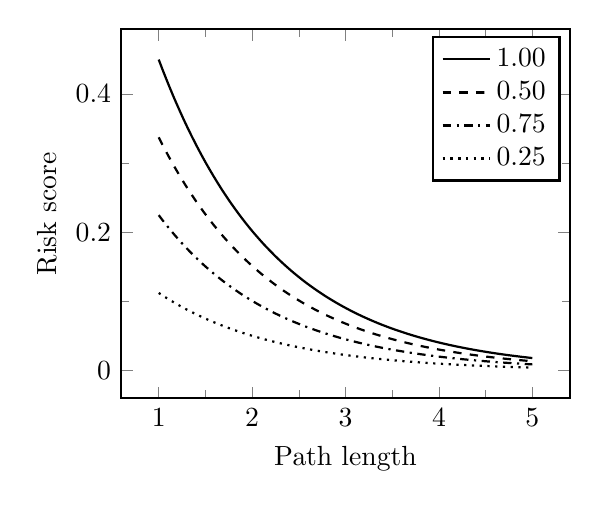
\begin{tikzpicture}
\begin{axis}[
  xlabel={Path length},
  ylabel={Risk score},
  minor tick num=1,
  width=0.6\textwidth,
  smooth,
  domain=1:5,
  y domain=0.01:1,
  samples=100,
  black,
  thick
]
  \addplot[] {e^(-0.8 * x)};
  \addplot[dashed] {0.75 * e^(-0.8 * x)};
  \addplot[dashdotted] {0.5 * e^(-0.8 * x)};
  \addplot[dotted] {0.25 * e^(-0.8 * x)};
  \legend{$1.00$, $0.50$, $0.75$, $0.25$};
\end{axis}
\end{tikzpicture}
\caption[Exponential decay of risk scores]{Exponential decay of risk scores.}
\label{fig:decay}
\end{figure}